\documentclass[]{article}

% Imported Packages
%------------------------------------------------------------------------------
\usepackage{amssymb}
\usepackage{amstext}
\usepackage{amsthm}
\usepackage{amsmath}
\usepackage{enumerate}
\usepackage{fancyhdr}
\usepackage[margin=1in]{geometry}
\usepackage{graphicx}
\usepackage{extarrows}
%\usepackage{setspace}
%------------------------------------------------------------------------------

% Header and Footer
%------------------------------------------------------------------------------
\pagestyle{plain}  
\renewcommand\headrulewidth{0.4pt}                                      
\renewcommand\footrulewidth{0.4pt}                                    
%------------------------------------------------------------------------------

% Title Details
%------------------------------------------------------------------------------
\title{Deliverable \#2 Template}
\author{SE 3A04: Software Design II -- Large System Design}
\date{}                               
%------------------------------------------------------------------------------

% Document
%------------------------------------------------------------------------------
\begin{document}

\maketitle	

\section{Introduction}
\label{sec:introduction}
% Begin Section



\subsection{Purpose}
\label{sub:purpose}
% Begin SubSection
The following document will outline the user interactions, architecture, and classes of the application, Nature Optix.  The intended audience for this document will be the teaching assistants as well as Dr. Ridha Kedhri. It is the goal of this document to provide insight to the intended audience into the internal mechanisms of Nature Optix. After reading this document, the audience should have a good understanding of the way in which a user can interact with the system, the architecture that the system uses, and the classes that comprise the system. 
% End SubSection

\subsection{System Description}
\label{sub:system_description}
% Begin SubSection
The Nature Optix application will allow the user to identify a natural phenomena. The application will ask the user a series of questions and the user will be able to specify an answer for each question from a drop down menu. The application will use a combination of repository and blackboard architecture. It will be comprised of 6 entities; 3 experts ( a physicist, a field expert, and a meteorologist), a location expert, a database corresponding to attributes identified by each one of the experts for every optical natural phenomena, and a controller. The database will contain all phenomena and information about the characteristics of each phenomena. Each expert will act as an algorithm that compares characteristics of a phenomena in the database to the user input. The physicist will compare the visual attributes, the field expert will compare the physical attributes, and the meteorologist will compare the weather condition attributes required for each phenomena to occur. Each expert will create a list of phenomena that has characteristics that match the user input. The three lists will then be sent to the controller. The controller will determine what phenomenon is common to all three lists and will present this phenomenon to the user. In some boundary cases, the applications shall provide the users with an aggregated list of closest match results to their query. The experts will not be able to communicate to each other and will only be communicating with the database and controller. 
% End SubSection

\subsection{Overview}
\label{sub:overview}
% Begin SubSection
The user interactions will be shown using a use case diagram, along with descriptions of each interaction.  The architecture for the system will be presented using descriptions along with justifications for decisions.  Furthermore, the classes of the application will be outlined using an analysis class diagram as well as a class responsibility collaboration. 
% End SubSection

% End Section

\section{Use Case Diagram}
%\label{sec:use_case_diagram}
\begin{figure}
	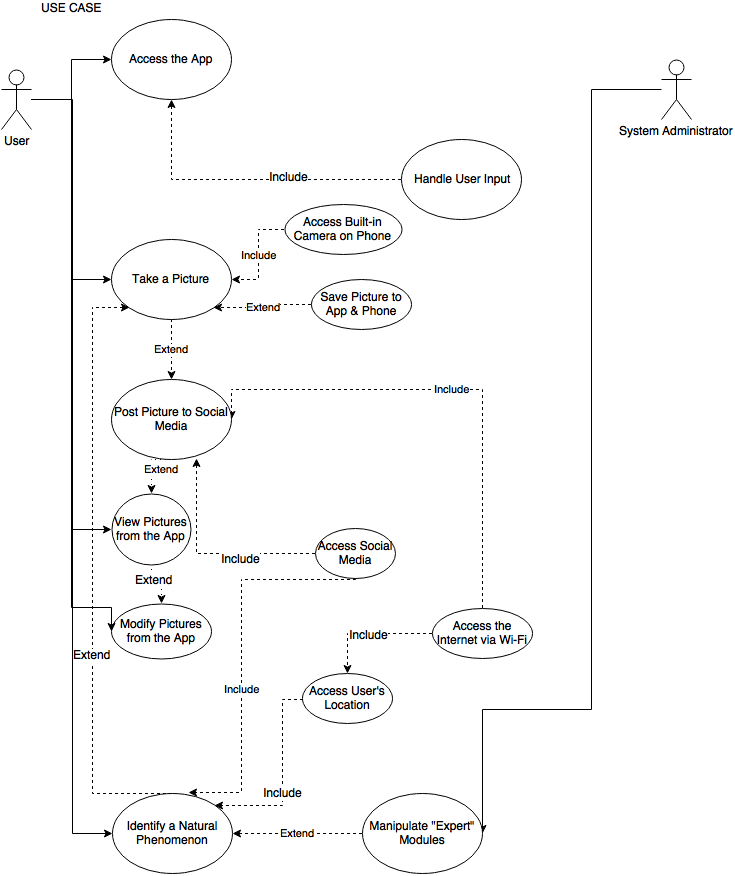
\includegraphics[width=\linewidth]{usecase.pdf}
	\caption{Use Case Diagram}
\end{figure}
\begin{enumerate}
	\item User wishes to access the app.  The user shall be able to download the app onto their smart phone in order to access it.  This downloading action will be handled by the operating system.  User shall be able to open the app.  The system developer needs to ensure that application shall be able to handle user input, so that the user can access and interact with the app.
	\item User wishes to take a picture and post it to social media.  User can then access the built-in camera on phone and it's functionality from the app.  User can also save the picture to the app and the phone if they so desire.  User shall be able to post to social media directly from the app.  The system developer shall ensure that application can access the internet via wireless connection from smart phone, the built-in camera on the smart phone, and social media (Instagram).  Application shall be able to save pictures directly to the phone.
	\item User wishes to view and modify pictures from the app.  User shall be able to view saved pictures through the app and the phone.  User shall be able delete pictures from the app and the phone.  System Developer shall ensure that application can display requested pictures to the user.  Application shall be able to delete pictures directly on the phone.
	\item User wishes to identify a natural phenomena. User shall be able to post a picture on social media through the app.  The system developer shall ensure that the app can access the user's location using google maps services. App shall have access to the internet via wireless connection from smart phone. App shall be able to switch "expert" modules in order to identify the natural phenomenon. 
\end{enumerate}
% End Section

\section{Analysis Class Diagram}
%\label{sec:analysis_class_diagram}
\begin{figure}
	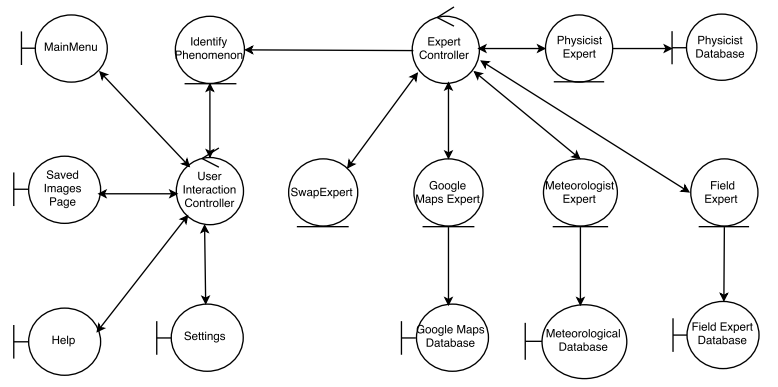
\includegraphics[width=\linewidth]{AnalysisClassDiagram.png}
	\caption{Analysis Class Diagram}
\end{figure}


\section{Architectural Design}
\label{sec:architectural_design}
% Begin Section
This section should provide an overview of the overall architectural design of your application. You overall architecture should show the division of the system into subsystems with high cohesion and low coupling.

\subsection{System Architecture}
\label{sub:system_architecture}
% Begin SubSection
\begin{enumerate}[a)]
	\item Identify and explain the overall architecture of your system
	\item We are using the Model-View-Controller architecture for our system.
	\item The Model View Controller hierarchy helps distinguish the business logic from the controller logic and is useful in creating modularity within the program. We are looking at this from 2 viewpoints:
		\item Our application is centered around displaying information to the user after they provide us with an initial input; the client will be focused on the view after the initial query which is handled by the model and finally connected by the controller to the view. Hence, an MVC architecture seems useful.
		\item MVC sets up our application to be enhanced further upon as it facilitates modular, high cohesion, low coupling design. We can add new modules without disrupting the existing codebase.
	\item Provide a structural architecture diagram showing the relationship among the subsystems (if appropriate)
\end{enumerate}
% End SubSection

\subsection{Subsystems}
\label{sub:subsystems}
% Begin SubSection
NatureOptix will be broken down into six subsystems. These subsystems are
\begin{enumerate}
	\item Controller %x2
	\item Experts x4,
	\item Database.
\end{enumerate}
The first Controller is the subsystem to control\begin{comment}ata between the user and the experts \end{comment} where the data goes. The controller will ask the user a series of questions. It will then take this information and pass it to the four experts. After the experts have returned with the potential answers to determine what phenomenon the user might be seeing, the controller will then present the options to the user. 

Three of the four Experts will be implemented as algorithms. These three experts are the Physicist, the FieldExpert, and the Meterologist. The experts will answer questions that pretain to their field. The Physicist will handle all physical aspects of natural phenomeon. This includes colour, shape, and size. The FieldExpert will be the expert responisble for identification based on attributes such as temperature and humidity. Finally the Meterologist will attempt to identify phenomeon based on the current weather at the location. The location expert will be the Google Maps API.

The final subsystem is the Database. Each expert will be assigned a Database. This ensures that the experts are easily swappable. The Database will store all the researched data about the natural phenomenon. Each expert will access the assigned database when needed. 
\begin{comment}
The second Controller will 
\end{comment}
% End SubSection

% End Section
	
\section{Class Responsibility Collaboration (CRC) Cards}
\label{sec:class_responsibility_collaboration_crc_cards}
% Begin Section
This section should contain all of your CRC cards.

\begin{enumerate}[a)]
	\begin{table}[ht]
		\centering
		\begin{tabular}{|p{5cm}|p{5cm}|}
		\hline 
		 \multicolumn{2}{|l|}{\textbf{Class Name: Database}} \\
		\hline
		\textbf{Responsibility:} & \textbf{Collaborators:} \\
		\hline
		Has information on all the phenomenons and each of their attributes. \vspace{1in} & \\
		\hline
		\end{tabular}
	\end{table}
	\begin{table}[ht]
		\centering
		\begin{tabular}{|p{5cm}|p{5cm}|}
		\hline 
		 \multicolumn{2}{|l|}{\textbf{Class Name: Expert1:Physicist}} \\
		\hline
		\textbf{Responsibility:} & \textbf{Collaborators:} \\
		\hline
		For attributes shape, colour, opacity, size, angle, elevation and brightness it will compare the attribute specifications given by the user to the phenomenons in the database and create a list of phenomenons that match the user input.  \vspace{1in} & Database, Controller \\
		\hline
		\end{tabular}
	\end{table}
	\begin{table}[ht]
		\centering
		\begin{tabular}{|p{5cm}|p{5cm}|}
		\hline 
		 \multicolumn{2}{|l|}{\textbf{Class Name: Expert2:FieldExpert}} \\
		\hline
		\textbf{Responsibility:} & \textbf{Collaborators:} \\
		\hline
		For attributes temperature, density and moistness it will compare the attribute specifications given by the user to the phenomenons in the database and create a list of phenomenons that match the user input. \vspace{1in} & \\
		\hline
		\end{tabular}
	\end{table}
	\begin{table}[ht]
		\centering
		\begin{tabular}{|p{5cm}|p{5cm}|}
		\hline 
		 \multicolumn{2}{|l|}{\textbf{Class Name: Expert3:Meterologist}} \\
		\hline
		\textbf{Responsibility:} & \textbf{Collaborators:} \\
		\hline
		For attributes sun, temperature and precipitation it will compare the attribute specifications given by the user to the phenomenons in the database and create a list of phenomenons that match the user input.\vspace{1in} & \\
		\hline
		\end{tabular}
	\end{table}
	\begin{table}[ht]
		\centering
		\begin{tabular}{|p{5cm}|p{5cm}|}
		\hline 
		 \multicolumn{2}{|l|}{\textbf{Class Name: Controller}} \\
		\hline
		\textbf{Responsibility:} & \textbf{Collaborators:} \\
		\hline
		Gives experts access to the database, and determines common phenomenons amongst the lists of the three experts and returns phenomenons to the user. \vspace{1in} & Expert1, Expert2, Expert3, GoogleAPI, Database\\
		\hline
		\end{tabular}
	\end{table}
	\begin{table}[ht]
		\centering
		\begin{tabular}{|p{5cm}|p{5cm}|}
		\hline 
		 \multicolumn{2}{|l|}{\textbf{Class Name: GoogleAPI}} \\
		\hline
		\textbf{Responsibility:} & \textbf{Collaborators:} \\
		\hline
		Determines users location to create list of phenomenons that could occur in the area that the user is in by comparing the location information to the location attribute in the database of phenomenons.\vspace{1in} & Database, Controller\\
		\hline
		\end{tabular}
	\end{table}
\end{enumerate}
% End Section

\appendix
\section{Division of Labour}
\label{sec:division_of_labour}
% Begin Section
Include a Division of Labour sheet which indicates the contributions of each team member. This sheet must be signed by all team members.
% End Section

\newpage
\section*{IMPORTANT NOTES}
\begin{itemize}
%	\item You do \underline{NOT} need to provide a text explanation of each diagram; the diagram should speak for itself
	\item Please document any non-standard notations that you may have used
	\begin{itemize}
		\item \emph{Rule of Thumb}: if you feel there is any doubt surrounding the meaning of your notations, document them
	\end{itemize}
	\item Some diagrams may be difficult to fit into one page
	\begin{itemize}
		\item It is OK if the text is small but please ensure that it is readable when printed
		\item If you need to break a diagram onto multiple pages, please adopt a system of doing so and thoroughly explain how it can be reconnected from one page to the next; if you are unsure about this, please ask about it
	\end{itemize}
	\item Please submit the latest version of Deliverable 1 with Deliverable 2
	\begin{itemize}
		\item It does not have to be a freshly printed version; the latest marked version is OK
	\end{itemize}
	\item If you do \underline{NOT} have a Division of Labour sheet, your deliverable will \underline{NOT} be marked
\end{itemize}


\end{document}
%------------------------------------------------------------------------------
